%% This is an example first chapter.  You should put chapter/appendix that you
%% write into a separate file, and add a line \include{yourfilename} to
%% main.tex, where `yourfilename.tex' is the name of the chapter/appendix file.
%% You can process specific files by typing their names in at the 
%% \files=
%% prompt when you run the file main.tex through LaTeX.
\chapter{Implementation}
During the thesis LSTM is used for predicting the future bounding box of the pedestrian using JAAD dataset. SSD is used as pedestrian detector. This chapter describes, how SSD is trained on large dataset, acquisition of data set and modeling LSTM on the JAAD dataset. Several aspect of Machine learning and Deep learning is discussed as well.

\section{LSTM - JAAD Dataset}
\subsection{Data Acquisition}
The early work includes prediction of road users behavior by employing dynamic factors e.g trajectory prediction, velocity prediction or predicting final goal of the pedestrian. JAAD dataset includes  behavioral aspect such as awareness by estimating head orientation along with other contextual information such as sign, weather condition, visibility and individual characteristics of the pedestrian such as things he carry, age and sex, size of the group he is associated with influence crossing behavior. JAAD is a publicly available large scale data set that includes data for pedestrian detection with behavioral and contextual information. It contains 346 video clips of pedestrian data that includes occlusion label, temporal correlation, behavioral aspect, contextual information weather related data.
In JAAD annotations are divided into 5 groups:
\begin{itemize}
	\item Annotations: Information about pedestrian bounding box, occlusion information, activities. These annotations are one per frame per label.
	\item Attribute: Contains information regarding pedestrian's crossing points, crossing characteristics. These annotations are one per pedestrian.
	\item Appearance: Information regarding pedestrian pose, clothing, objects they carry. These information are one per frame per pedestrian.
	\item Traffic: Includes information about traffic signs, traffic light for each frame.
	\item Vehicle: Per frame vehicle speed information e.g moving fast, speeding up.
\end{itemize}

The pedestrians\' actions are categorized into 3 groups: \\
Precondition- this refers to the state of the pedestrian prior to crossing and can be either standing, moving slow or fast. \\
Attention- the way the pedestrian becomes aware of the approaching vehicle. These actions, depending on their duration, are looking ( > 1s) or glancing ($\leq$ 1s). \\
Response- this includes the behaviors that pedestrians exhibit in response
to the action of the approaching vehicle, namely, stop, clear path, slow down, speed up, hand gesture and nod.
Occlusion information is provided in the form of tags for each bounding box: partial occlusion (between 25\% and 75\% visible) and full occlusion (less than 25\% visible).  654 unique pedestrian samples (out of 2.2k samples) with behavioral tags in the dataset. 

\subsection{Data preparation}
\cite{rasouli2017agreeing} Rasouli et al. provided a supporting GitHub code for easier interaction with JAAD data. The videos can be downloaded by running the script \colorbox{lightgray}{download\textunderscore clips.sh}. The video clips are downloaded into JAAD\textunderscore clips and the clips are named as below.\\
\colorbox{lightgray} {JAAD\textunderscore clips/video\textunderscore  0001.mp4} \\
\colorbox{lightgray} {JAAD\textunderscore clips/video\textunderscore  0002.mp4}

Using \colorbox{lightgray}{split\textunderscore clips\textunderscore to\textunderscore .sh} the frames are extracted to corresponding video id directory with in a folder called \textit{images} \\
\begin{center}
\colorbox{lightgray} {images/video\textunderscore  0001/0000.png} \\
\colorbox{lightgray} {images/video\textunderscore  0001/0001.png} \\
\colorbox{lightgray} {....}
\end{center}

%https://github.com/ykotseruba/JAAD/issues/7
The video data and image data was used to manual exploration of data set and was not used for LSTM training. For LSTM training annotations from JAAD was extracted for videos 71-346. These are the videos recorded with Garmin GDR-35 with dimension 1920x1980.\footnote{videos 1-60: GoPro Hero+ (1920x1980)
videos 61-70: Highscreen Box Connect (1280x720) information received from author of JAAD paper ykotseruba}. Widely used python packages such as \textit{numpy }and \textit{pandas} are used for transform and manipulation of dataset. NumPy is a scientific computing package specializing array operations and Pandas provides high performance ease to use data analysis tool using python programming language.  \\

\begin{algorithm}[H]
\SetAlgoLined
\KwResult{Set of csv files containing bounding box information }
 initialize JAAD path and video set for bb information are to be extracted \;
 \While{video in video set}{
  fetch the relevant information from json\;
  \eIf{video length < 90}{
   discard such entries\;
   }{
	 fetch the bb information from json data-structure
   write the bb information to corresponding csv file\;
  }
 }
~\\
~\\
 \caption{Algorithm for BB data preparation}
\end{algorithm}

It is noticed that there are limited number of videos for some of the scenario and for other scenarios there are more number of videos. To avoid data-skew impacting the final result, the videos are watched and stored in categorized directory. After taking the frequencies of videos in category, factors are determined  and used  replication factor during preparation of training data for the LSTM. The training sequence for the LSTM is prepared as follows.

\begin{algorithm}[H]
\SetAlgoLined
\KwResult{train\textunderscore X, val\textunderscore X: training and validation sequences for the model }
 initialize the path for different category and and replication factor to be considered \;
 \While{csv file in file set}{
  fetch the relevant information from json\;
	normalize and fit the co-ordinates using MinMaxScaler\;
	form a series of sequence taking number of input and number of future step\;
	append all such series and prepare a large structure 
 }
reshape to the desired shape\;
80 percentage of the prepared data is stored into train\textunderscore X\;
20 percentage of the prepared data is stored into val\textunderscore X\; 
~\\
~\\
 \caption{Algorithm for LSTM training data preparation}
\end{algorithm}

\textbf{Note:} MinMax scalar at a global scale introduce the error, because several video clips are taken from a very close distance to the object and several other video clips are recored from a far distance. To mitigate this issue \textit{MinMax scalar } for every video clip was created and the data sequence is transformed and fit in accordance to that.

\subsection{Training }
Once training data is prepared, the next step is to fit the model with data taking validation data as a guiding factor. During my work, Keras- LSTM APIs are used for the modeling. The below algorithms are used for the source code implementation.\\
\begin{algorithm}[H]
\SetAlgoLined
\KwResult{Save the better model and it's weights after each training iteration}
 initialize the model check pointing using ModelCheckpoint class with relevant parameters\;
 // monitor='val\textunderscore loss' is used to select better model\;
	use model check pointing as a callback\;
 //design network\;
 clear\textunderscore session\;
 model = Sequential()\;
 model.add(LSTM(50, input\textunderscore =(train\textunderscore X.shape[1], train\textunderscore X.shape[2]))) \;
 // dropout avoids over fitting \;
 model.add(Dropout(0.1))\; 
 model.add(Dense(4))\;
 model.compile(loss='mae', optimizer="adam")\;
 epochs = 300\;
 // fit network\;
 // The model tries to fit the weights by iterating the training \\
 // dataset for 'epoch' number of time, monitors the validation loss  \\
 // when validation loss is better than previous, that model weights are saved
 history = model.fit(train\textunderscore X, train\textunderscore y, \\
 \HS \HS \HS \HS epochs=epochs, \\
 \HS \HS \HS \HS batch\textunderscore size=72,\\
 \HS \HS \HS \HS validation\textunderscore data=(val\textunderscore X, val\textunderscore y),\\
 \HS \HS \HS \HS verbose=2,\\
 \HS \HS \HS \HS callbacks=callbacks,\\
 \HS \HS \HS \HS shuffle=False)
~\\
~\\
\caption{Algorithm for LSTM training using Keras API} 
\end{algorithm} \label{training-algo}

Once the model is trained for a particular number of epochs, model training performance can be visualized by plotting a graph and the best model can be saved using below pseudo-code. \\

\begin{algorithm}[H]
\SetAlgoLined
\KwResult{Plot the training-validation graph and saves the best model with weights}
 The model is generated using \ref{training-algo} \;
 // history variable is updated \\
 // use history to plot the training loss and validation loss using pyplot\;
 pyplot.plot(history.history['loss'], label='train')\;
 pyplot.plot(history.history['val\textunderscore loss'], label='test')\;
 pyplot.legend()\;
 pyplot.savefig("char-file-name.png")\;
 pyplot.show()\;

// save model\;
model.save("{}.h5".format(lstm-model-name)) \;
~\\
~\\
 \caption{Algorithm for plotting the graph and saving the model} 
\end{algorithm}

\subsection{Framework parameters}
% https://datascience.stackexchange.com/questions/20413/clarification-on-the-keras-recurrent-unit-cell
For the LSTM model number of units for the cell is used as 50, which determines the learning capacity of the model. A dropout of 0.1 is used to avoid over fitting, model is trained for  300 number of epochs. A batch size of 72 is used. Mean absolute Error (\textit{mae}) is used as the loss function and Adaptive Moment Estimation (\textit{adam}) is used as the optimizer. The Keras's default values for adam's parameter are used. The default value for \textit{learning rate} is 0.01 and \textit{decay} is 0.0001. 

\section{SSD model}

\subsection{Data Acquisition}
Challenges are there while just considering image data, the verities of image sources for example we can get photos that are taken by professionals, synthetic photos drawn by image generators and real life photos that we see and capture in our day to day life. So the results of these benchmarks and 
observation across these aforementioned classes of data set does not transfer to the other scenarios.
As recommended always for machine learning tasks, we should consider real data as close as possible to the environment where the designed system is expected to work. And luckily there exist some excellent data set in the public domain. I chose Caltech Data set \cite{dollar2009pedestrian}, which is one of the latest data set available in the public till today. 

\newpara
This data set contains highly annotated video, recorded from a moving vehicle in a normal trafic situation. It contains pedestrians vary largely in appearance, pose and scale. It also includes occlusion information. It contains close to 10 hours of recording at 30 fps with a video resolution 640 x 480. As seen and mentioned by the authors the overall image quality lower than that of same image resolution. The data set includes ~350,000  pedestrian bounding boxes (BB) labeled in 250,000frames and remains the largest such data set to  date. As already mentioned by \cite{walk2010new} Caltech data set is difficult for various reasons.

\begin{itemize}
	\setlength\itemsep{-1em}
	\item Many small pedestrians
	\item realistic occlusion frequency
	\item image quality is poor
	\item includes blur
	\item visible JPEG artifacts
\end{itemize}

\subsection{Data preparation}
After the video data got acquired, with help of a publicly available python project \cite{shuntasaito2015}, the original annotations in \textit{MATLAB} compatible \textit{vbb} format is converted to a JSON structure for easier consumption. The generated json file further processed and required data is extracted into a csv file using a python script located at \url{ https://github.com/Kalinga/ML/blob/master/ssd_keras_caltech/json_anno_csv_conversion.ipynb}. As mentioned by \cite{dollar2009pedestrian} the video set from 00-05 is expected for training purpose and 06-10 is for testing purpose.

In the Caltech data group of people are separately label as \textit{people}. With the intention, the ML model should learn individual person and identify persons rather than people, when there are several persons close by, i decided to remove \textit{people} class label from the training data set. And also the number of samples for \textit{people} and \textit{person} was disproportionately varying. This was another reason to exclude \textit{people }label from  the training. 
%The frequency for the both classes are shown as below.

%\begin{figure}[H]
%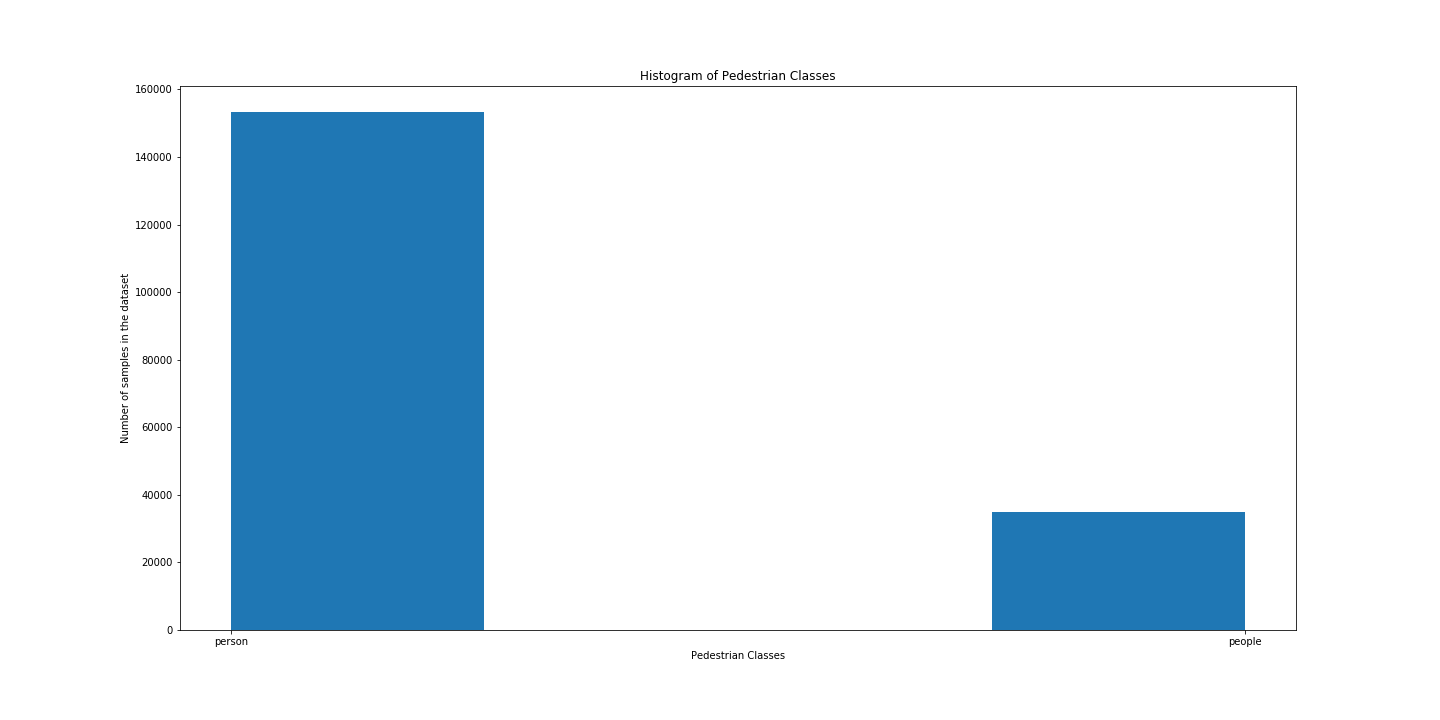
\includegraphics[scale=0.4]{classid_distribution1_2}
%\begin{center}
%\caption{Class 'person' and 'people' distribution}
%\end{center}
%\end{figure}

As per \cite{walk2010new}, unoccluded pedestrians with 50-pixel-or-taller are considered , as they are not clear. For simplicity purpose below data are discarded from the training set.
\begin{itemize}
	\item Class label with \textit{people}, \textit{person-fa}, \textit{person?}
	\item occluded \textit{person} label
	\item images below 50 pixel in height
	\item images below 5 pixel in width
\end{itemize}

After the above mentioned clean up, our training data contains total 48194 number of BB with person as a label in 26902 unique frames and sample data looks as below:
\begin{center}
\texttt{  \\
frame,xmin,xmax,ymin,ymax,class\textunderscore id \\
set00\textunderscore V000\textunderscore 1213.png,573,591,169,211,1 \\
set00\textunderscore V000\textunderscore 1213.png,473,484,170,193,1 \\
set00\textunderscore V000\textunderscore 166.png,406,418,164,187,1 \\
set00\textunderscore V000\textunderscore 166.png,435,442,167,181,1 \\
set00\textunderscore V000\textunderscore 166.png,233,241,120,134,1 \\
set00\textunderscore V000\textunderscore 744.png,564,588,153,218,1 \\
set00\textunderscore V000\textunderscore 744.png,565,587,173,206,1 \\
set00\textunderscore V000\textunderscore 654.png,406,417,162,194,1 \\
}
\end{center}

During the training an NVIDIA GeForce GTX 1080 GPU with 8GB of video memory was used, while using a validation data size equals to standard 10\% of training data, the training time was equals to unusable, as training of a single epoch was taking nearly ~30-40 hours. The experiment was run on a shared Linux server hosted within the University Network and the computing resource was shared with other students. Keeping this in view, i decided to reduce the size of the validation data set size to great extent and get an approximate impression about the model's training efficiency. Below table show the training and validation data partition.

\begin {table}[H]
\begin{center}
 \begin{tabular}{||c c c||}
 \hline
 Data Set & Bounding Box & Frames\\ [0.8ex] 
 \hline\hline
 Training & 47194 & 26280 \\
 \hline
 Validation & 1000 & 622 \\
 \hline
 Total & 48194 & 26902 \\
 \hline
\end{tabular}
\caption{Training and Validation sample numbers}
\end{center}
\end {table}

\cite{dollar2009pedestrian} defines pedestrians with 80 pixels or taller as in the near scale and 30 pixel or less
are in the far scale and rest in the medium scale. Most pedestrians are observed in medium scale. A person with 1.8m tall is 1.5s away from the vehicle for the mentioned set up and speed of 55km\/h. \cite{dollar2011pedestrian} shows that average aspect ratio \textit{$w \approx 0.41h$}. After above mentioned cleaning steps, a re calculation for the aspect ration distribution shows, it does not vary much from the original distribution, as shown below.

\begin{figure}[H]
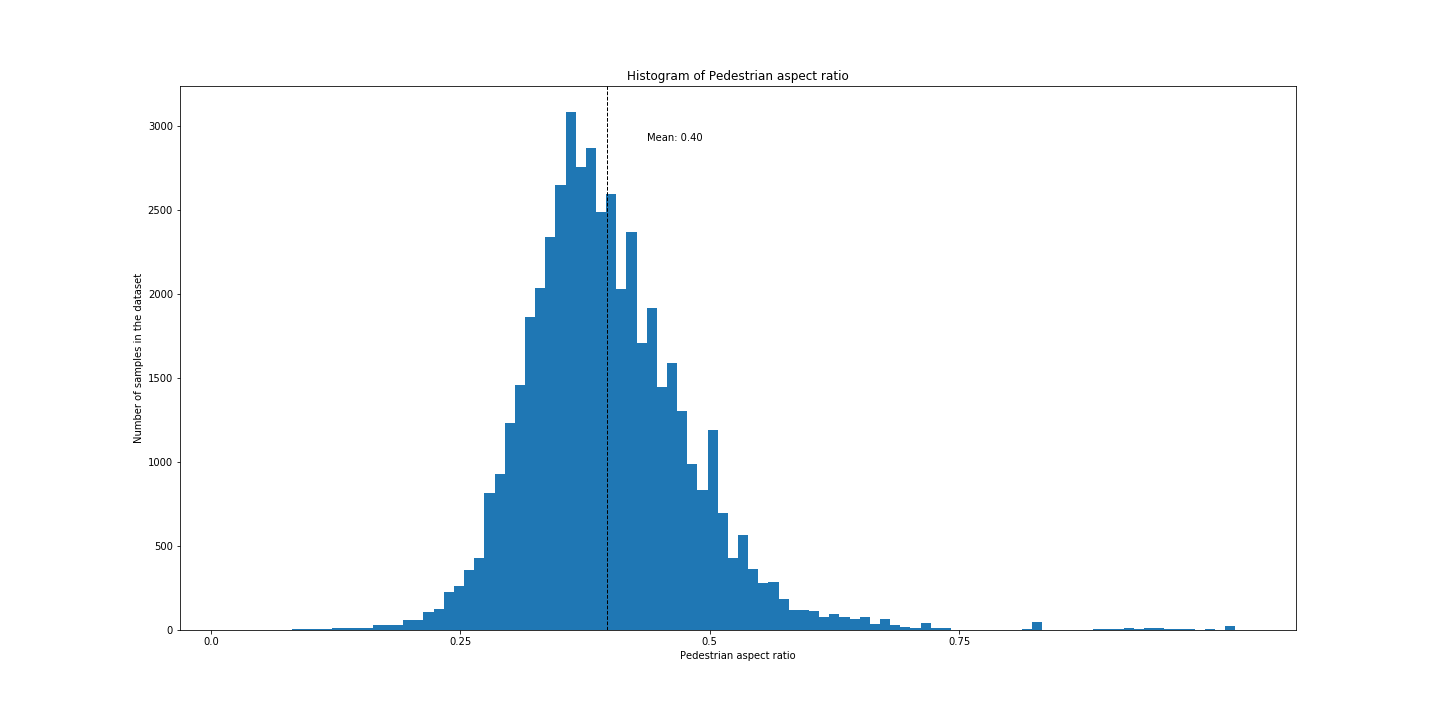
\includegraphics[scale=0.4]{aspect_ratio_distribution}
\begin{center}
\caption{Pedestrian aspect ratio distribution}
\end{center}
\end{figure}

\subsection{Training }
As SSD has predictors at multiple level, before the model training step, a pre-processing step is required where proposed BBs are generated and compared with the ground truth and depending on IoU threshold, certain prior BBs are considered and encoded for the training purpose. There are several parameters play a role in generating bounding boxes and some of critical parameters used are given below.

\subsection{Framework parameters}

\begin {table}[H]
\begin{center}
 \begin{tabular}{||c c||} 
 \hline
 Param. Name & Value\\ [0.8ex] 
 \hline\hline
 img\textunderscore  height & 480 \\ 
 \hline
 img\textunderscore  width & 640 \\
 \hline
 img\textunderscore  channels & 3 \\
 \hline
 n\textunderscore  classes & 1 \\
 \hline
 scales & $[0.08, 0.16, 0.32, 0.64, 0.96]$ \\
 \hline
\end{tabular}
\caption{SSD framework parameters}
\end{center}
\end{table}

\subsection{Model parameters}
\textbf{Model Architecture:}
SSD model consists of convolutional feature layers and some convolutional predictor layers that take input from different feature layers, making the model fully convolutional. In the presented model, 7 convolutional layers and 4 predictors layers are used. These 4 convolutional predictors layers take input from layers 4, 5, 6, and 7 respectively. convnet with was used for modeling using keras \footnote{Keras is a high-level neural networks API, written in Python and capable of running on top of TensorFlow, CNTK, or Theano.}. The model is created and initialised with Keras API Sequential (). 

\subsection{Hyper Parameters}
 
%--------AS IS---------------
%Creating a layer of LSTM memory units allows you to specify the number of memory units within the layer.
%Each unit or cell within the layer has an internal cell state, often abbreviated as “c“, and outputs a hidden state, often abbreviated as “h“.
%-----------------------
